\documentclass[options]{article}

% paquetes
\usepackage[spanish]{babel}
\usepackage{graphicx}

\title{Práctica del Tema 5: Publicación y difusión}
\author{Blanca María Pérez Soriano}

\begin{document}
\maketitle
\begin{abstract}
    \begin{center}
        Creación y publicación de un modelo 3D a partir de un modelo digitalizado representado como una nube de puntos
    \end{center}   
\end{abstract}

\pagebreak

\section{Preparación}
\subsection{Software}
%TODO: meter meshlab en un link a su página principal
Para realizar esta práctica utilizaremos el programa MeshLab en la versión 64bit v2023.12.

\subsection{Modelo de puntos}
Para la realización de esta práctica se utilizará el modelo de nube puntos proporcionado en el recurso \textit{"Modelos para la práctica"}: \textbf{MayanSculpture.ply}.

\subsection{Importación a MeshLab}
%TODO: sustituir y poner el nombre modelo que se va a utilizar
Para importar el modelo de nube de puntos seleccionado seguiremos las siguientes acciones: \textbf{File → Import Mesh → MayanSculpture.ply}
\begin{center}
    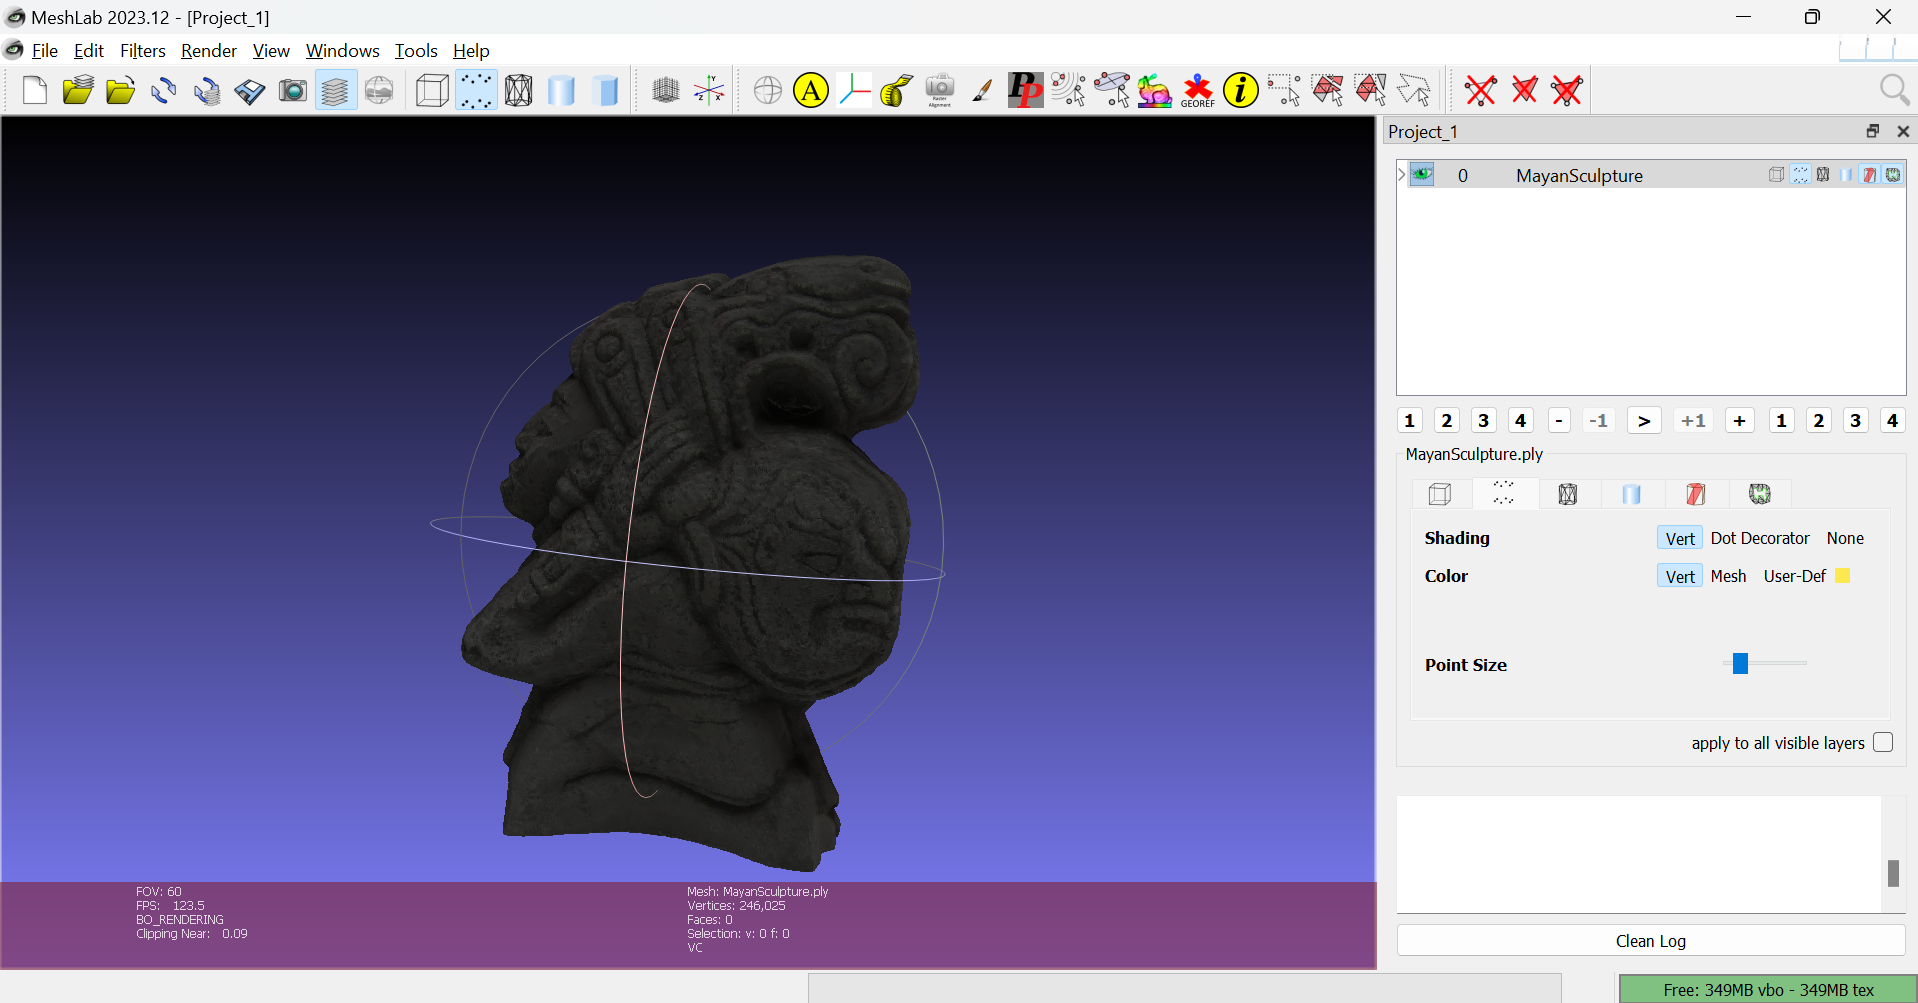
\includegraphics[scale=0.35]{images/presentacion_importacion.png}    
\end{center}

\pagebreak

\section{Resolución de la práctica}
\subsection{Triangulación}

\subsection{Utilización de GitHub}

\textbf{GitHub} es una plataforma de colaboración en proyectos de software, apoyada en \textbf{Git}, lo cual nos permite llevar, además, un \textit{control de versiones} de los documentos que vayamos publicando en el repositorio. 


Para crear un repositorio y hacer seguimiento de este proyecto haremos click, dentro de nuestro panel principal, en \textbf{\textit{"New"}}:

\begin{center}
    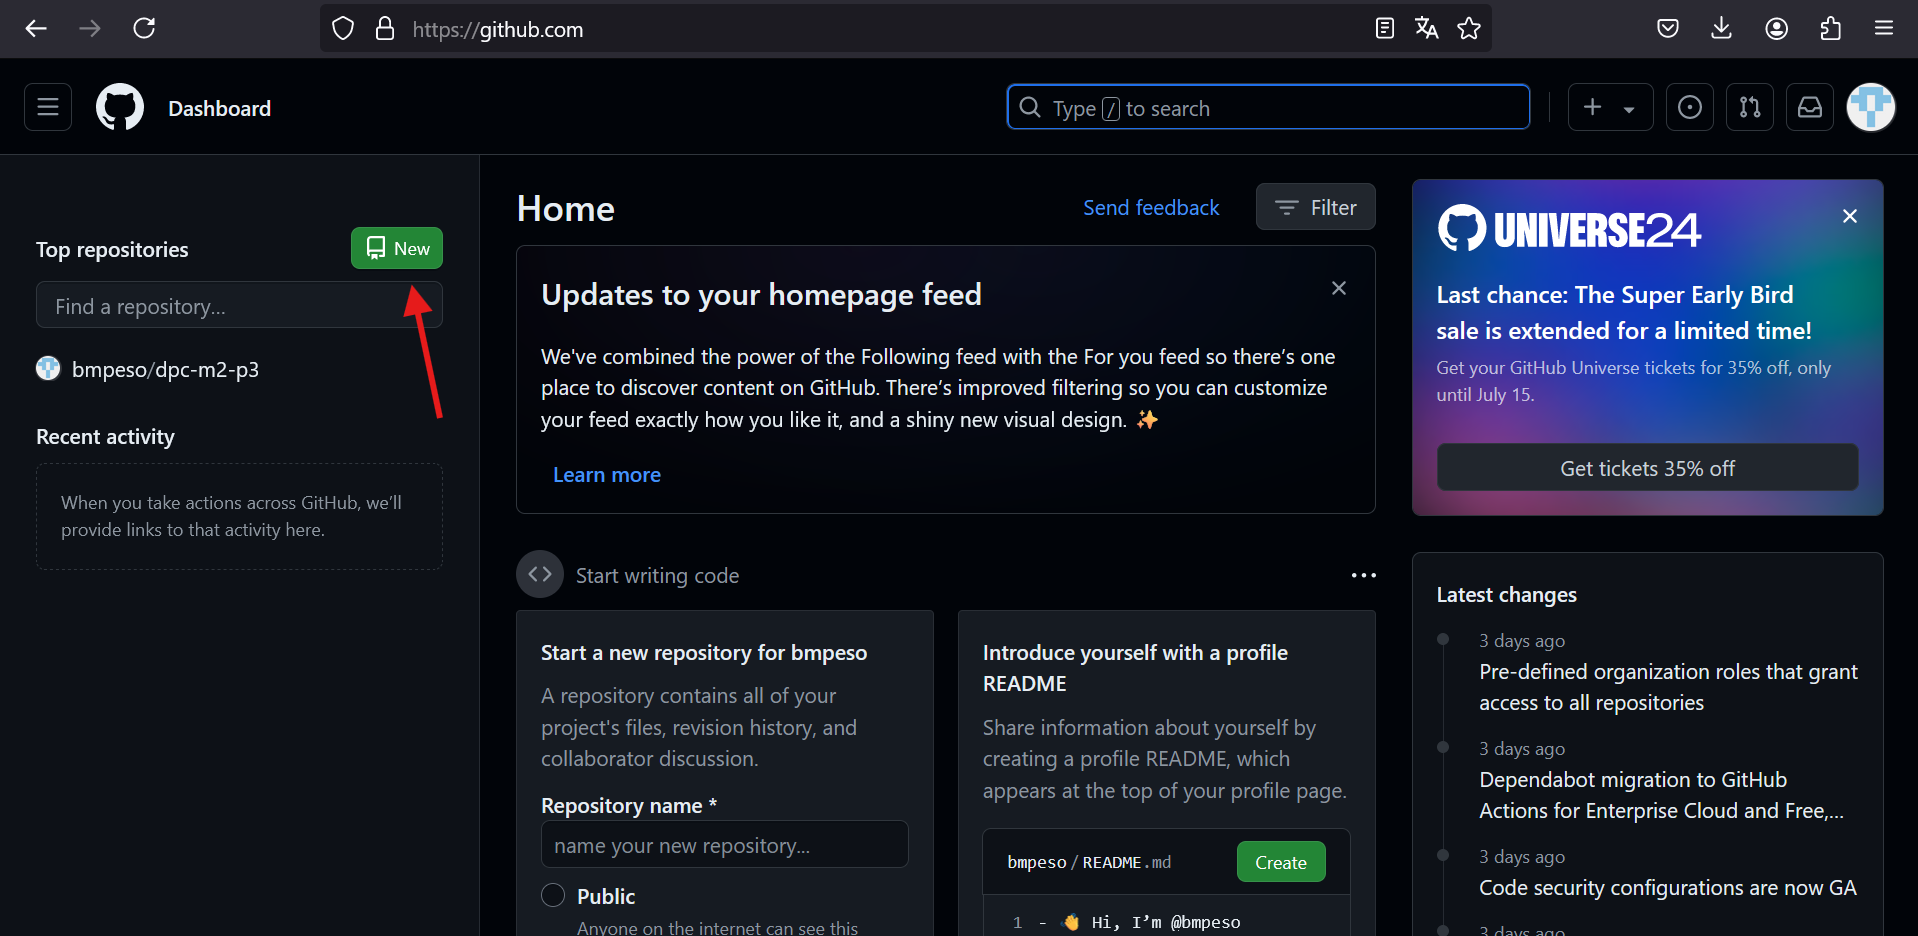
\includegraphics[scale=0.35]{images/github_01.png}
\end{center}

A continuación rellenaremos los campos que creamos convenientes \textit{(señalo en recuadros los campos modificados)} y haremos click en \textbf{\textit{Create repository}}:

\begin{center}
    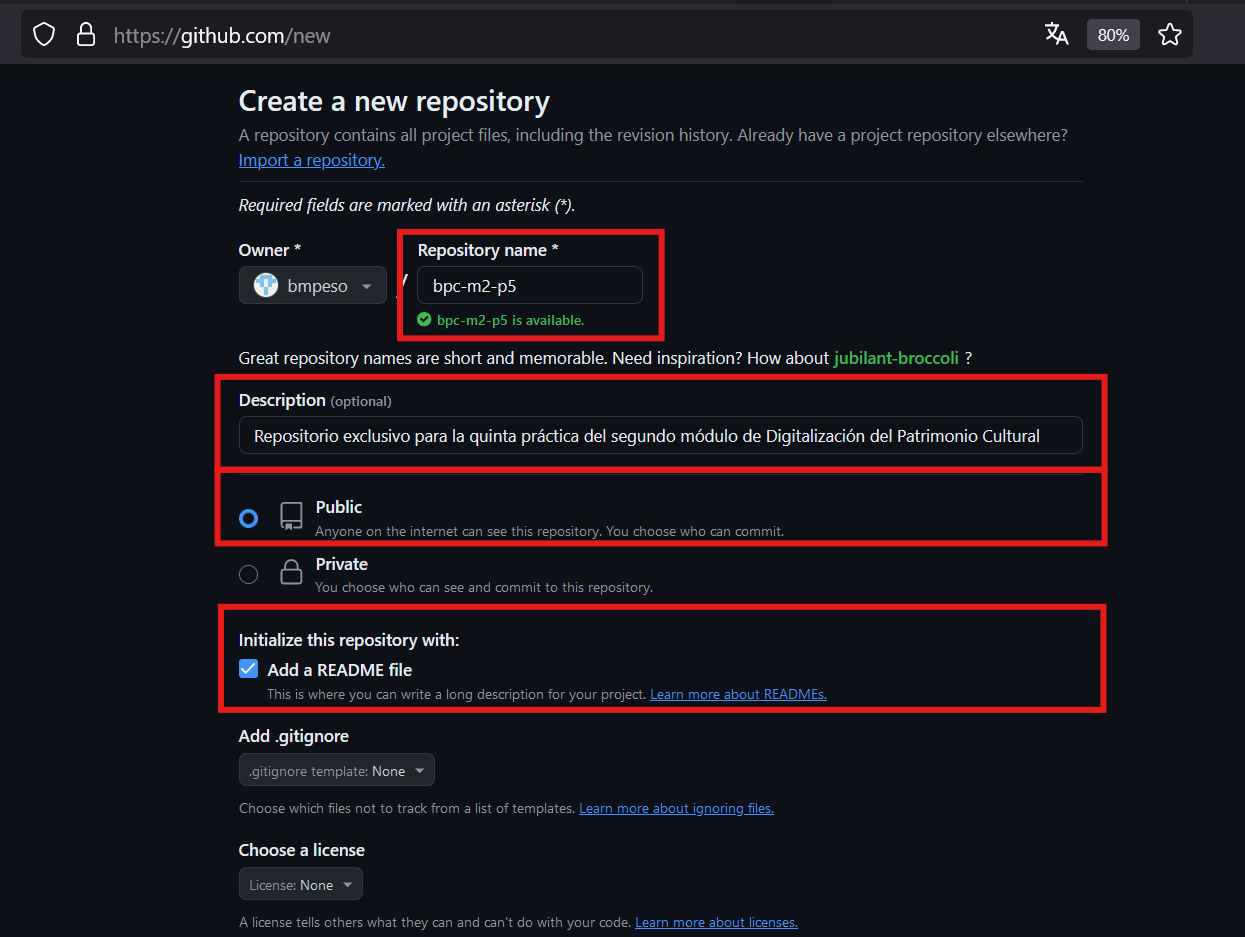
\includegraphics[scale=0.45]{images/github_02.png}
\end{center}

\end{document}